\chapter{Korišteni algoritmi i matematički aparat}

\section{Funkcije gubitka}

Gubitak je funkcija koja nam govori koliko nam je model dobar u predviđanju na skupu za učenje. Njega nastojimo minimizirati nekim od optimizacijskih postupaka. Postoje različite vrste gubitaka koje nam mogu dati različite rezultate za isti model. Neke od najpoznatijih funkcija gubitaka su: Unakrsna entropija (engl. Cross Entropy) i Negativna log izglednost (engl. Negative log likelihood). Minimizacija gubitka je iterativan postupak koji svakom iteracijom pomiče parametre modela u smjeru smanjenja gubitka.

\subsection{Negativna log-izglednost}
	Negativna log-izglednost je gubitak izražen formulom:
	\[
		L = -\sum_{i}log P(Y = y_i | \textbf{x}_i)
	\]
	$P(Y = y_i | \textbf{x}_i)$ je vjerojatnost da se podatak $\textbf{x}_i$ klasificira u razred $y_i$.
	Tu vjerojatnost računamo pomoću softmaxa. Softmax je funkcija koja "spljošćuje" ocjenu svakog podatka na interval [0,1].
	\[
	S : \mathbb{R} \mapsto [0,1]
	\]
	\[
	S(f_{y_i}) = \frac{e^{f_{y_i}}}{\sum_{j} e^{f_j}}
	\]
	Ovakva formulacija nam osigurava da će suma svih softmaksa primijenjenih na ocjene biti 1. Iz slike \ref{fig:NLL} vidimo kako negativna log-izglednost penalizira male vjerojatnosti, dok je za vjerojatnosti koje su blizu 1 gubitak približan nuli.
	\begin{figure}[H]
		\centering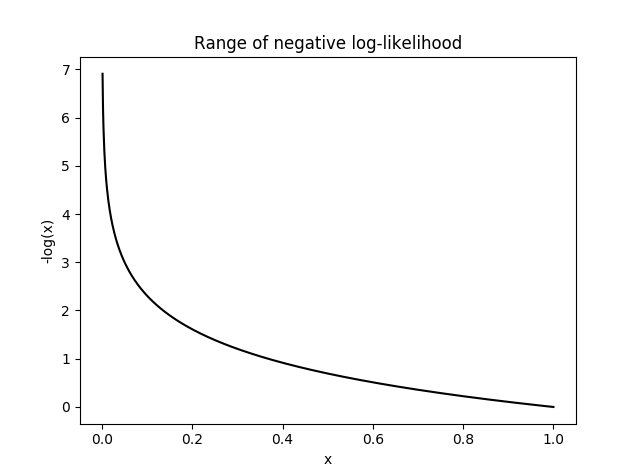
\includegraphics[scale=0.5]{slike/neg_log.png}
		\caption{NLL [\cite{miranda2017softmax}]}
		\label{fig:NLL}
	\end{figure}

\subsection{Udaljenost od naučenih središta}
	Udaljenost od naučenih središta je gubitak izražen formulom:
	\[
		L_c = \frac{1}{2} (x_i-c_k)^2
	\]
	\[
		c_k = \frac{1}{N_k}\sum_{y_i=k}f_{y_i}^1(x_i)
	\]
	$c_k$ - središta klasa
	\newline
	$x_i$ - podatak
	\newline
	$f_{y_i}^1(x_i)$ - izlazi iz mreže
	\newline
	
Ovaj gubitak nastoji minimizirati udaljenosti izlaznih podataka od središta pripadnih razreda. Posljedica tog pristupa je bolje grupiranje podataka koji pripadaju istom razredu. Najčešće se koristi u kombinaciji s nekim drugim gubitkom npr. negativnom log-izglednosti, pri čemu se utjecaj ovog gubitka skalira nekim parametrom radi stabilnosti. Ovakav pristup smo odabrali u projektu te funkcija gubitka izgleda ovako.
\[
	L = L_n + \lambda L_c
\]
 Ovaj gubitak pokazuje najbolje rezultate u slučaju kad podatci za učenje sadrže mali broj slika po razredu, a veliki broj razreda. [\cite{centerloss}]
	 


\section{Unazadna propagacija}

Unazadna propagacija je matematički algoritam korišten u učenju neuronskih mreža bez povratnih veza. Cilj algoritma je odrediti koliko svaki primjerak za učenje utječe na težinske parametre mreže. Rezultat algoritma je nužan za promjenu tih težina kako bi povećali aktivaciju bitnih neurona, odnosno smanjili aktivaciju manje bitnih neurona.\\\\Model možemo matematički predstaviti kao funkcijsku kompoziciju:
	\[g(x):=f^{L}(W^{L}f^{L-1}(W^{L-1}\cdots f^{1}(W^{1}x)\cdots ))\]
	gdje je \(x\) ulaz, \(g(x)\) predviđeni izlaz, \(f^l\) aktivacijska funkcija sloja \(l\) te \(W^l\) matrični zapis težina između slojeva \(l\) i \(l-1\)
	
	\noindent\\Učenje modela se svodi na minimizaciju funkcije gubitka neuronske mreže. Za pronalazak globalnog minimuma funkcije koristi se negativni gradijent. Algoritmom se računa gradijent spomenute funkcije gubitka za svaki primjerak za učenje. Izračun uzima u obzir trenutne težinske parametre mreže.
	
	\[C(y,g(x))\]
	\[C(y,f^{L}(W^{L}f^{L-1}(W^{L-1}\cdots f^{2}(W^{2}f^{1}(W^{1}x))\cdots )))\]
	\(C\) je funkcija gubitka, \(y\) je željeni izlaz.
	
	\noindent\\Funkcija gubitka se lančanim pravilom derivira po \(a^l\) koji predstavlja izlazak iz aktivacijskog sloja \(l\).
	\[{\frac {dC}{da^{L}}}\cdot (f^{L})'\circ W^{L}\cdot (f^{L-1})'\circ W^{L-1}\cdots (f^{1})'\circ W^{1}\]
	\(\circ\) označava Hammardov produkt.
	
	\noindent\\Gornji izraz se transponira te se redoslijed množenja članova okrene. Dobiveni izraz predstavlja traženi gradijent.
	\[\nabla _{x}C=(W^{1})^{T}\cdot (f^{1})'\ldots \circ (W^{L-1})^{T}\cdot (f^{L-1})'\circ (W^{L})^{T}\cdot (f^{L})'\circ \nabla _{a^{L}}C.\]
	
	\noindent\\Dobiveni gradijent je vektor čije vrijednosti možemo dovesti u bijektivni odnos sa težinama mreže. Interpretacija tih vrijednosti je iznos za koji primjerak za učenje želi promjeniti određenu težinu.
	
	\noindent\\Iz izraza za gradijent se sada može odrediti gradijent za pojedini sloj \(l\). Označimo sa \(\delta ^{l}\) gradijent ulaznih vrijednosti u sloj \(l\). 
	\[\delta ^{l}:=(f^{l})'\circ (W^{l+1})^{T}\cdots \circ (W^{L-1})^{T}\cdot (f^{L-1})'\circ (W^{L})^{T}\cdot (f^{L})'\circ \nabla _{a^{L}}C.\]
	
	\noindent\\Gradijent ulaznih vrijednosti u sloj \(l\) se može zapisati rekurzivno.
	\[\delta ^{l-1}:=(f^{l-1})'\circ (W^{l})^{T}\cdot \delta ^{l}.\]
	
	\noindent\\Sada se može izraziti za bilo koju razinu \(l\).
	
	$$\delta ^{1}\&=(f^{1})'\circ (W^{2})^{T}\cdot (f^{2})'\cdots \circ (W^{L-1})^{T}\cdot (f^{L-1})'\circ (W^{L})^{T}\cdot (f^{L})'\circ \nabla _{a^{L}}C$$
					
				$$\delta ^{2}\&=(f^{2})'\cdots \circ (W^{L-1})^{T}\cdot (f^{L-1})'\circ (W^{L})^{T}\cdot (f^{L})'\circ \nabla _{a^{L}}C$$
				
				$$\vdots$$ 
				
				$$\delta ^{L-1}\&=(f^{L-1})'\circ (W^{L})^{T}\cdot (f^{L})'\circ \nabla _{a^{L}}C$$
				
				$$\delta ^{L}\&=(f^{L})'\circ \nabla _{a^{L}}C,$$
		
		\noindent\\Gradijent težina za određeni sloj \(l\) se sada izražava kao:
		\[\nabla _{W^{l}}C=\delta ^{l}(a^{l-1})^{T}.\]
		\noindent\\Na kraju algoritma težine modela se ažuriraju sloj po sloj (od zadnjeg prema prvom) u skladu s tim vrijednostima.  


\section{Optimizatori}

Optimizacija je jedan od ključnih dijelova u procesu treniranja modela. Njezina svrha je minimizirati pogrešku generalizacije nad skupom kojim treniramo.
Kad govorimo o optimizaciji, najkorištenija metoda je svakako gradijentni spust, no korištenjem njega se mogu manifestirati neki problemi koji kao posljedicu imaju nepronalazak optimalnih težina. Postojanje više lokalnih minimuma i spora kovergencija jedni su od problema. Stoga je naš izbor bio SGD i ADAM optimizator. 

Stohastički gradijentni spust (SGD) za razliku od običnog gradijentnog spusta neće pasti na nulu prilikom pronalaska lokalnog ili globalnog minimuma, a razlog leži u tome što SGD procjenjuje iznos gradijenta i posljedično stvara šum.
Stohastički gradijenti spust koristili smo uz momentum koji ubrzava učenje. 

Adaptive Moment Estimation (ADAM) je optimizator koji kombinacijom dvije metodologije gradijentnog spusta momentuma i RMSprop algoritma ubrzava pronalazak globalnog minimuma. Glavna značajka ADAM-a je što koristi prosječno eksponencijalno kretanje gradijenta i kvadratnog gradijenta, te ga to čini izrazito efikasnim na velikim skupovima podataka i
u radu s velikim brojem parametara. 